\chapter{Fundamentação Teórica}
\label{cap:2fundamentacao}
Neste capítulo serão apresentados os conceitos
abordados neste trabalho. O problema inverso será apresentado
em linhas gerais e a inversão sísmica será abordada em maiores detalhes.
Serão apresentados os conceitos relacionados a \textit{Deep Learning}, assim como os
elementos de redes neurais convolucionais. Esta fundamentação
teórica é relevante para o entendimento de como o modelo de rede neural convolucional
pode ser adotado para obter ganho qualitativo e quantitativo no pós-processamento
da inversão sísmica.

\section{Problema Inverso}

A teoria de inversão é utilizada em diversas áreas para inferir os valores de
parâmetros relacionados com processos físicos a partir de um conjunto de dados medidos,
os quais são chamados dados experimentais. É possível descrever o problema inverso
como o processo de obter informações de um sistema parametrizado, a partir de
dados que podem ser medidos por meio de algum experimento físico e das relações teóricas com os parâmetros
desejados, mas que não são passíveis de medição. Frequentemente, algum conhecimento \textit{a priori}
é incorporado ao modelo.

Um sistema físico depende do domínio em estudo. Pode ser uma galáxia para um
astro-físico, pode ser a Terra para um geofísico ou uma partícula quântica
para um físico quântico. Em comum, o fato de que, para ser estudado, um sistema
físico segue três passos básicos: a parametrização do sistema, a modelagem direta e a modelagem inversa \cite{tarantola}.
A parametrização do sistema se refere à definição do conjunto mínimo de elementos (parãmetros, variáveis)
cujos valores caracterizam completamente o sistema.
%Como mencionado no Capítulo \ref{cap:1intro},
%a modelagem direta se refere à definição das leis físicas que permitem realizar previsão
%de dados observáveis, a partir de valores dos parâmetros do modelo. A modelagem inversa,
%por sua vez, se caracteriza pelo uso de resultados atuais das medições dos parâmetros
%físicos observáveis, para inferir os valores atuais dos parâmetros do modelo (não-observáveis).

A modelagem direta significa prever os valores dos parâmetros observáveis (dados $d$),
que correspondem a um dado modelo (conjunto de parâmetros $m$). Esta predição pode ser denotada
pela Eq. \ref{eq:frdmdl}. Onde $F(.)$ é chamado operador direto.
\begin{equation}
\label{eq:frdmdl}
F(m) = d 
\end{equation}

Por sua vez, a modelagem inversa se refere ao uso de resultados atuais das medições dos parâmetros
físicos observáveis, para inferir os valores atuais dos parâmetros do modelo (não-observáveis).
O problema inverso pode ser descrito em uma forma discreta como:
\begin{equation}
\label{eq:deqgm}
m = F^{-1}(d)
\end{equation}
onde, F é o sistema físico investigado, e relaciona os parâmetros do modelo $m=(m_1, m_2,...,m_n) \subset R^n$
estimado com os dados observados $d \in R^s$.
Como mencionado no Capítulo \ref{cap:1intro}, um problema inverso possui múltiplas soluções,
de modo que o modelo $m$ pertence a um conjunto de modelos $M$ admissíveis.
Na prática, $d$ pode ser uma função no domínio do tempo e/ou espaço, ou pode ser
uma coleção de observações discretas.

\section{Inversão Sísmica}

Os métodos geofísicos frequentemente envolvem a solução e avaliação de problemas inversos,
pois permitem inferir a distribuição das propriedades físicas na subsuperfície da Terra
usando observações da superfície. A inversão sísmica tem um papel fundamental na solução 
de problemas geofísicos, em especial na caracterização de reservatórios \cite{Bosch2010} \cite{Srivastava2009}.
Do ponto de vista prático, as soluções para o problema de inversão sísmica melhoram a exploração e
o gerenciamento na indústria petrolífera, uma vez que os dados sísmicos estimados possuem forte correlação com as
propriedades petrofísicas (porosidade, densidade, etc.) das rochas da subsuperfície \cite{Figueiredo2014}.
Para facilitar o entendimento da inversão sísmica, considere a subsuperfície como sendo formada por camadas
sobrepostas de diferentes tipos de rochas. As regiões onde ocorrem as transições entre tipos
diferentes de rochas são comumente chamadas de \textit{facies} e podem ter espessuras diferentes.

\subsection{Aquisição Sísmica}
O dado sísmico é o principal parâmetro observável utilizado na inversão sísmica.
A aquisição destes dados se dá por meio da sísmica de reflexão. Este
método utiliza pulsos sísmicos de uma fonte artificial controlada e monitora a resposta em
função do tempo. Neste sistema, cada região de contato entre dois tipos de rochas
diferentes gera reflexão e refração do pulso sísmico, como demonstrado na Figura
\ref{fig:1sismica}.
De um ponto de vista bastante elementar, é possível intuir que a parte refletida da onda se
propaga em todas as direções, de modo que os componentes horizontal e vertical podem ser medidos.
O componente horizontal (\textit{s-wave}), referente à reflexão horizontal
da onda, é utilizado no processo de inversão conhecido como inversão elástica. Por outro lado, o componente
vertical da onda (\textit{p-wave}), referente à reflexão vertical do pulso emitido, é utilizado no processo
conhecido como inversão acústica.
\begin{figure}[ht!]
\begin{center}
  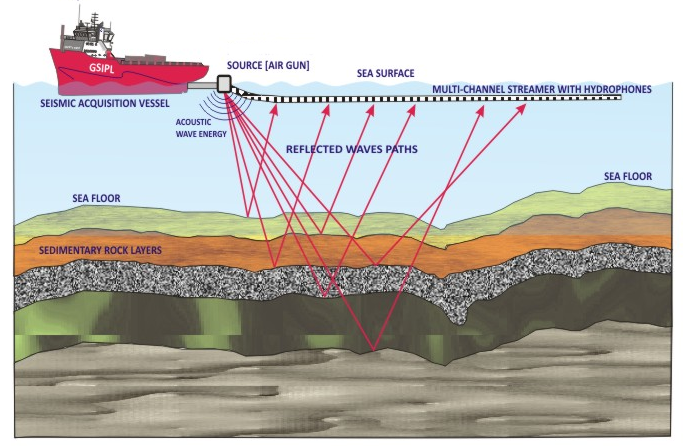
\includegraphics[width=0.8\textwidth]{fig/seismic_survey_2}
  \caption{Método de sísmica de reflexão \citep{figsismica}}
  \label{fig:1sismica}
\end{center}
\end{figure}

O pulso de onda emitido durante a aquisição possui um formato próprio, uma identidade, 
conhecido como \textit{wavelet}. Assim, a resposta sísmica medida
é composta em parte por esta identidade e, em parte, pela característica da interface
entre duas camadas de rochas diferentes, na qual o pulso reflete.
Esta característica é chamada de coeficiente de refletividade (equação \ref{eq:refletv}):
\begin{equation}
r(t) = \frac{z(t+\delta t)-z(t)}{z(t+\delta t)+z(t)}
\label{eq:refletv}
\end{equation}
onde, $z(t)$ é a impedância acústica no tempo $t$ definida por
$z(t)=\rho(t)v(t)$, onde $\rho(t)$ é a densidade da rocha e $v(t)$ a
velocidade de propagação da onda acústica.
O dado sísmico utilizado na inversão acústica, portanto,
é uma aproximação da resposta da camada terrestre. Pode ainda ser definido como
a convolução entre a \textit{wavelet} de aquisição e o valor de refletividade entre as
camadas, com ângulo de incidência e reflexão de $90^\circ$,
respectivamente. Por este motivo, este modelo é chamado convolucional.
Com os coeficientes de reflexão e a discretização da medida de tempo, é possível
modelar o dado sísmico $d(t)$ aplicando a convolução $\otimes$
da \textit{wavelet} $s$ com os coeficientes de refletividade $r$:
\begin{equation}
d(t) = s(\tau) \otimes \sum_{j-1}^{N}{r(t- t_j) \delta(t - t_j) + e_d(t)}
\end{equation}
onde $N$ é o número total de camadas, $e_d(t)$ representa o ruído aleatório em função do tempo
e cada $d_{xy}$ é chamado de traço sísmico. Um conjunto de traços
sísmicos também é chamado de imagem, seção ou cubo, no caso de um
levantamento 3D. A \textit{wavelet} ideal seria um pulso tipo delta contendo
todas as frequências, entretanto, na prática as
\textit{wavelets} são pulsos de banda limitada entre $6Hz$ e $65Hz$, o que
limita a frequência da sísmica e sua resolução \citep[p. 11]{sen_livro}.
Como consequência, as imagens resultantes do processo de inversão também terão
o seu espectro de frequência limitado. A Figura \ref{fig:wavelet} ilustra uma
\textit{wavelet} típica extraída de dados reais.
\begin{figure}[htp]
\begin{center}
  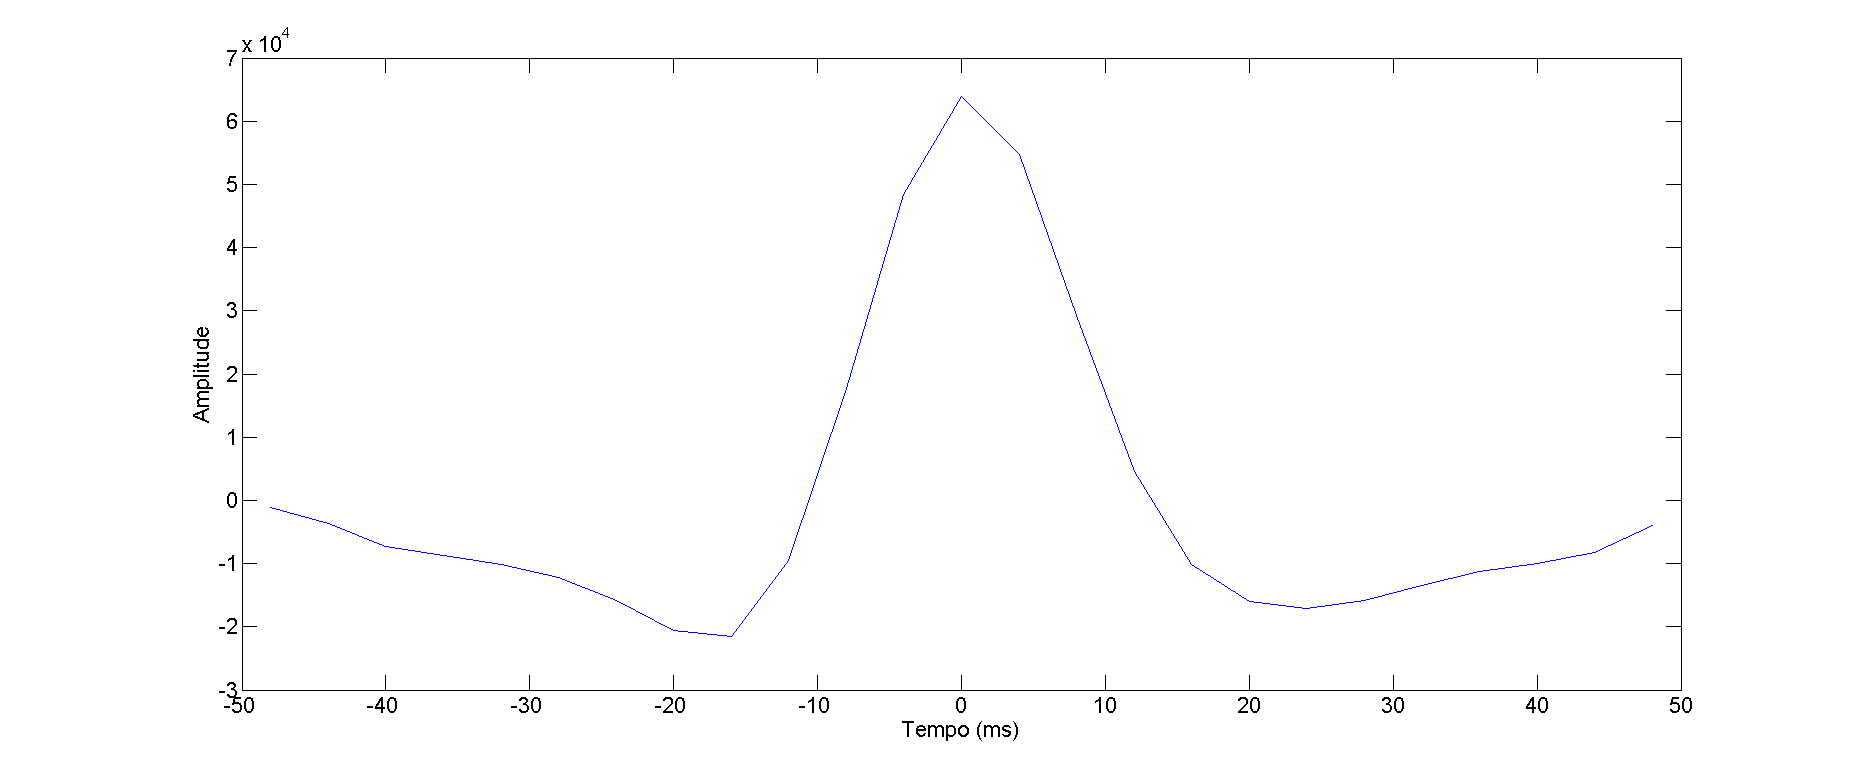
\includegraphics[width=0.8\textwidth]{fig/wavelet}
  \caption{\textit{Wavelet} extraída de dados reais}
  \label{fig:wavelet}
\end{center}
\end{figure}

%%
Falta explicar como ocorre a inversão.
\subsection{Inversão Sísmica Linear e Não Linear}

\subsection{Máximo \textit{a posteriori}}

\section{Redes Neurais Convolucionais}
As Redes Neurais Convolucionais (CNN), também chamadas de redes convolucionais,
são um tipo de rede neural especializada em processamento de dados que possuem uma
topologia conhecida e em forma de grade \cite{Gdfl16}. Exemplos deste tipo de dado são as séries
temporais, que podem ser vistas como uma grade em uma dimensão (1-D) com amostras
em intervalos regulares de tempo, e dados de imagem, que podem ser vistos como
uma grade (2-D) de \textit{pixels}. Este modelo de rede neural é chamada convolucional,
pois emprega a operação de convolução no lugar de multiplicação comum entre matrizes,
em pelo menos uma de suas camadas.

\subsection{Convolução}
A operação de convolução é definida como a integral do produto de duas funções após uma delas sofrer um
certo deslocamento. Considere o exemplo em que se deseja rastrear a localização de uma
nave espacial com um sensor a lazer. O sensor disponibiliza uma saída $x(t)$ referente à posição da nave
no tempo $t$. Ambos, $x$ e $t$, são valores reais, de modo que uma saída diferente pode ser obtida
em qualquer instante de tempo. Considerando que o sensor possui um certo ruido, para realizar uma
estimativa mais precisa da posição da nave é preciso ponderar várias medidas de posição juntas.
Como os valores medidos mais recentemente são mais relevantes, se estima uma função peso
$w(a)$, onde $a$ é o tempo de medição. Se esta média ponderada for aplicada a todos os instantes,
a estimativa de posição da nave será suavizada:

\begin{equation}
 s(t) = \int{x(a) w(t-a)da}
 \label{eq:1}
\end{equation}

Esta operação é chamada convolução e pode ser definida para quaisquer
funções, às quais a integral da equação \ref{eq:1} esteja definida. A convolução
costuma ser denotada com um asterisco e aplicada com o tempo $t$ discretizado para valores inteiros:
\begin{equation}
 s(t) = (x * w)(t) = \sum_{a=-\infty}^{\infty}{x(a)w(t-a)}
 \label{eq:2}
\end{equation}

No contexto das redes convolucionais, $x$ se refere ao conjunto de imagens de entrada 
e $w$ é denominado \textit{kernel} ou filtros. As imagens de entrada são uma sequência multidimensional 
de dados, enquanto os filtros são uma sequência multidimensional de parâmetros a serem 
otimizados pelo algoritmo de aprendizagem.
Nos casos em que o problema compreende imagens $X$ e filtros $W$ utilizados em duas dimensões 
a convolução ganha o seguinte formato:

\begin{equation}
 S(i,j) = (X*W)(i,j) = \sum_{m}\sum_{n}{X(m,n)W(i-m,j-n)}
\end{equation}

Nas redes convolucionais há pelo menos duas estruturas básicas, a camada convolucional e a camada de \textit{pooling}.
A arquitetura típica de uma CNN compreende duas camadas convolucionais, cada uma das quais é seguida por
uma camada \textit{pooling}, como ilustrado na Figura \ref{fig:cnn_basic_arq}. À medida que as imagens progridem
ao longo da rede, suas dimensões diminuem, entretanto, elas se tornam mais profundas
em termos de hierarquia de conceitos extraídos. No topo da pilha de camadas da rede
se adiciona camadas completamente conectadas, sendo que, na última camada ocorre a saída prevista.
Esta estrutura de camadas completamente conectadas é a mesma utilizada nas redes neurais tradicionais
do tipo \textit{feedforward}, nas quais todos os nerônios de uma camada estão conectados a todos os
neurônios da camada seguinte. 
\begin{figure}[htp]
\begin{center}
  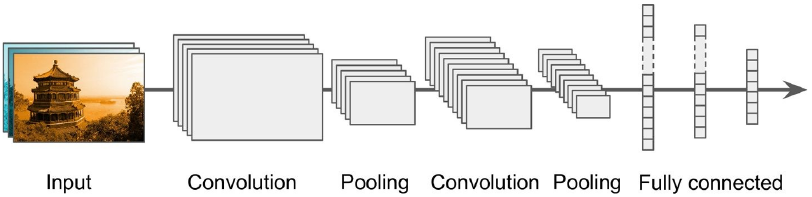
\includegraphics[width=0.8\textwidth]{fig/cnn_basic_arq}
  \caption{Arquitetura típica de uma rede neural convolucional. Fonte:\cite{aurelien17}}
  \label{fig:cnn_basic_arq}
\end{center}
\end{figure}

A camada convolucional é o elemento mais importante de uma CNN. Esta camada é estruturada
de modo a fazer com que cada um dos seus neurônios esteja conectado a um 
pequeno grupo de \textit{pixels} da camada de entrada (Figura \ref{fig:cnn_arq}) e não a todos os \text{pixels}, como
ocorre em redes neurais tradicionais. Cada neurônio da camada seguinte se conecta apenas aos neurônios
contidos em uma pequena região da camada anterior e assim sucessivamente. Esta região que define
o grupo de neurônios conectados ao neurônio da próxima camada é chamada \textbf{campo perceptivo}.
Este formato permite o aprendizado de características de baixo nível na primeira camada e de
características de mais alto nível nas camadas seguintes.
\begin{figure}[htp]
\begin{center}
  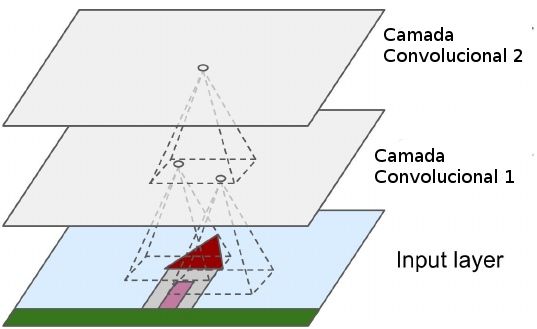
\includegraphics[width=0.8\textwidth]{fig/cnn_arq}
  \caption{Camadas de uma CNN com campos receptivos retangulares.}
  \label{fig:cnn_arq}
\end{center}
\end{figure}

A Figura \ref{fig:cnn_stride} ilustra a conexão entre as camadas de uma rede convolucional.
Considere um neurônio localizado na linha $i$ e coluna $j$ de uma dada camada.
Este neurônio estará conectado às saídas dos neurônios da camada anterior
localizados nas linhas $\times{i}{s_h}$ até $\times{i}{s_h}+f_h - 1$, colunas
$\times{j}{s_w}$ até $\times{j}{s_w}+f_w - 1$, onde
$f_h$ e $f_w$ são a altura e a largura do campo receptivo, $s_h$ e $s_w$
são os deslocamentos vertical e horizontal ao longo das imagens da camada anterior.
O tamanho destes deslocamentos é chamado de passo ou \textit{stride}
e quanto maior o \textit{stride}, menor será a imagem resultante na camada seguinte. Para \textit{stride}
de tamanho $0$ a camada seguinte terá as mesmas dimensões da camada anterior.
\begin{figure}[htp]
\begin{center}
  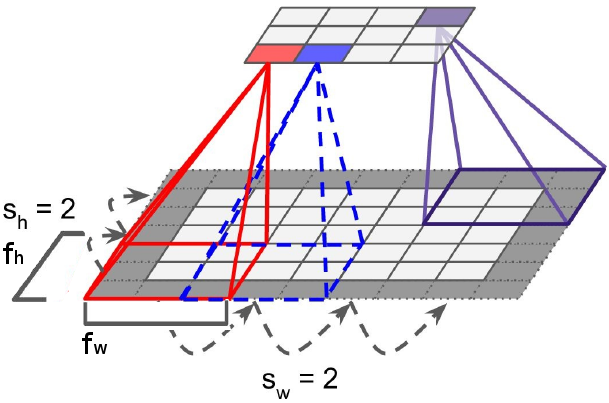
\includegraphics[width=0.8\textwidth]{fig/cnn_layer_stride_2}
  \caption{Conexão entre camadas com campo receptivo 3 x 3 e \textit{strides} de tamanho 2.}
  \label{fig:cnn_stride}
\end{center}
\end{figure}

\subsection{Filtros}
Os filtros (pesos) em uma camada convolucional são representados como uma pequena
imagem com as mesmas dimensões do campo receptivo. São eles os elementos
convolvidos com a imagem de entrada para obter o resultado da camada convolucional.
A Figura \ref{fig:conv_filt} ilustra dois conjuntos de filtros possíveis. O primeiro filtro é um quadrado preto
(\textit{pixels} de valor 0) contendo uma coluna central branca (\textit{pixels} com valor 1). 
Analogamente, o segundo filtro é um quadrado preto contendo uma linha central branca.
É possível notar na imagem da esquerda que as linhas verticais brancas se tornaram mais
evidentes, enquanto as outras partes da imagem se tornaram mais borradas. De modo análogo, na imagem da direita 
a convolução com o filtro horizontal destacou as linhas brancas horizontais, ao passo que
o restante ficou borrado. Assim, uma característica detectada por um neurônio representa
o tipo de padrão da entrada que causará a sua ativação.
Estes padrões podem ser bordas, contornos ou estruturas com outras formas.
\begin{figure}[htp]
\begin{center}
  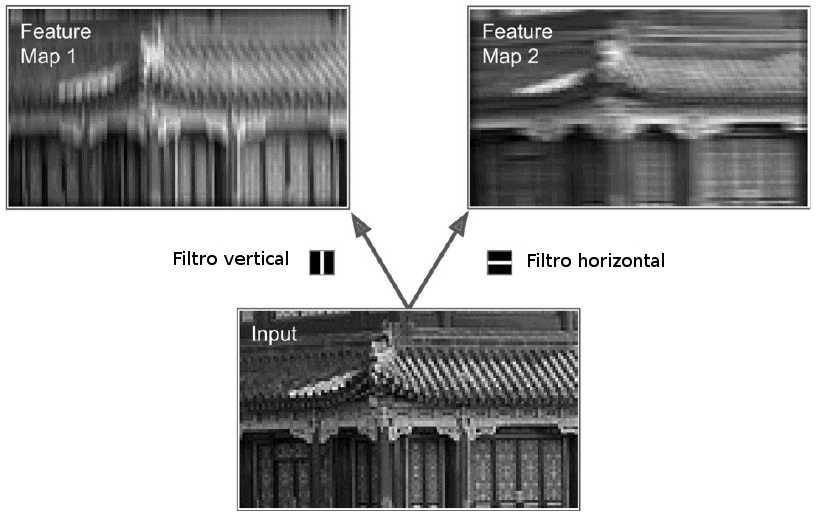
\includegraphics[width=0.7\textwidth]{fig/conv_filt}
  \caption{Aplicação de dois filtros diferentes para obter mapas de características.}
  \label{fig:conv_filt}
\end{center}
\end{figure}

Em situações reais, a camada convolucional possui muitos mapas de características, resultando
em uma representação em 3-D como ilustrado na Figura \ref{fig:featmaps}. Os mapas de características
de uma camada convolucional são o resultado da convolução de uma das imagens de entrada com os diversos
filtros específicos desta camada. Na Figura \ref{fig:featmaps} estão ilustrados os mapas para a convolução
com apenas uma imagem, de modo que é possível imaginar que, à medida que o número de imagens aumenta,
a estrutura ilustrada se replica horizontalmente. 
\begin{figure}[htp]
\begin{center}
  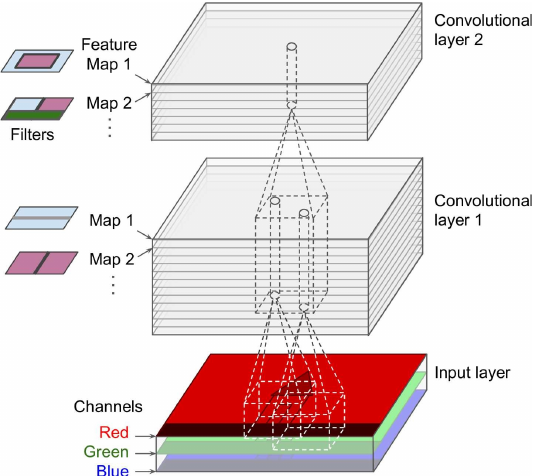
\includegraphics[width=0.7\textwidth]{fig/feat_maps}
  \caption{Camadas convolucionais com múltiplos mapas de características e imagens com três canais.}
  \label{fig:featmaps}
\end{center}
\end{figure}

\subsection{Pooling}
Uma camada em uma rede convolucional consiste de três estágios. No primeiro estágio,
a camada realiza diversas convoluções para produzir um conjunto de ativações lineares.
O segundo estágio é chamado etapa de detecção, na qual cada ativação é submetida a uma
função não-linear. A terceira etapa é chamada de \textit{pooling}, responsável por
modificar a saída para o resumo estatístico das saídas em uma determinada vizinhança. A operação de
\textit{pooling} permite tornar invariante pequenas translações no conjunto de entrada,
ou seja, ainda que haja pequenas translações na entrada, os valores da maioria das saídas após a
o \textit{pooling} permanecem iguais. A Figura \ref{fig:pool} ilustra o funcionamento da função de \textit{pooling}.
\begin{figure}[htp]
\begin{center}
  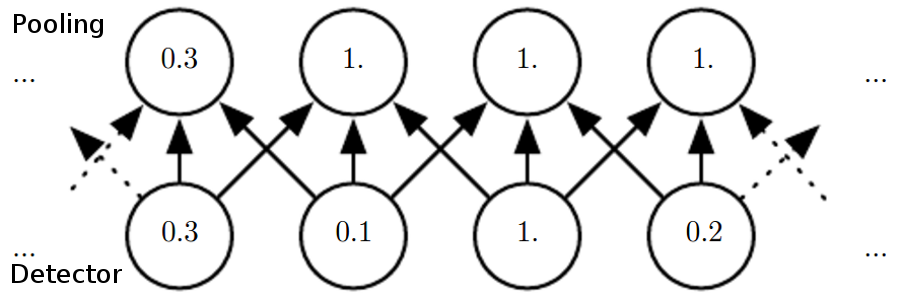
\includegraphics[width=0.7\textwidth]{fig/pool}
  \caption{Operação de \textit{pooling} com região de tamanho 3. Nesta operação é selecionado o máximo valor de ativação da etapa de detecção.}
  \label{fig:pool}
\end{center}
\end{figure}

A operação de \textit{pooling} permite lidar com entradas de tamanho variável.
Classificar imagens de tamanhos diferentes, por exemplo, pode ser realizado
variando o tamanho entre as regiões de \textit{pooling} de modo que a camada de 
de classificação sempre receba o mesmo número de sumários estatísticos
independente do tamanho da imagem.

\subsection{Propriedades das Redes Convolucionais}
Por conta da sua arquitetura, as redes convolucionais se sustentam sobre três pilares: interações esparsas, compartilhamentos
de parâmetros e representações equivariantes. As propriedades de interação esparsa e compartilhamento de pesos serão apresentadas
com maior nível de detalhes nesta seção, embora já tenham sido introduzidos de forma intuitiva nas seções anteriores.

As O \textbf{interações esparsas}, também chamadas de conectividade esparsa ou pesos esparsos,
ocorre quando os filtros possuem  dimensão menor que a entrada, ou seja a
dimensão do campo receptivo é menor que a dimensão das imagens de entrada.
De um ponto de vista prático, a imagem de entrada pode ter milhares de \textit{pixels}, entretanto, é 
possível detectar apenas pequenas regiões com características de maior relevância na imagem de entrada
com filtros que compreendam apenas algumas dezenas ou centenas de \textit{pixels}.
Por exemplo, é possível identificar características de uma face humana na identificação de pessoas, ou estruturas com
significado geológico em um estudo geofísico. Como consequência,
menos parâmetros são armazenados e há um ganho na eficiência estatística do
modelo. As Figuras \ref{fig:sparse} e \ref{fig:full} ilustram
os modelos de conectividade esparsa e tradicional, respectivamente.
É possível notar que na conectividade tradicional (Figura \ref{fig:full}) todos os elementos da camada inferior
afetam o elemento em destaque $s_3$ da camada seguinte, enquanto na conectividade esparsa (Figura \ref{fig:sparse}) apenas
três elementos afetam o elemento em destaque. O número de elementos que afetam o elemento em destaque na
conectividade esparsa é definido pelo tamanho do filtro utilizado na convolução.

\begin{figure}[htp]
\begin{subfigure}{.5\textwidth}
  \centering
  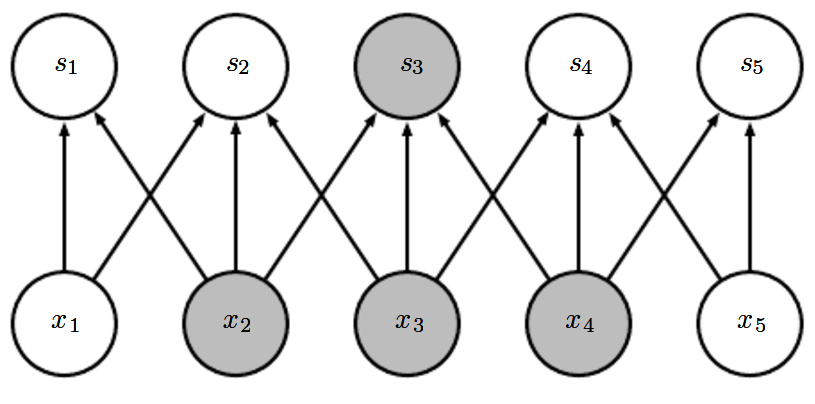
\includegraphics[width=.9\linewidth]{fig/sparse}
  \caption{Conectividade esparsa.}
  \label{fig:sparse}
\end{subfigure}
\begin{subfigure}{.5\textwidth}
  \centering
  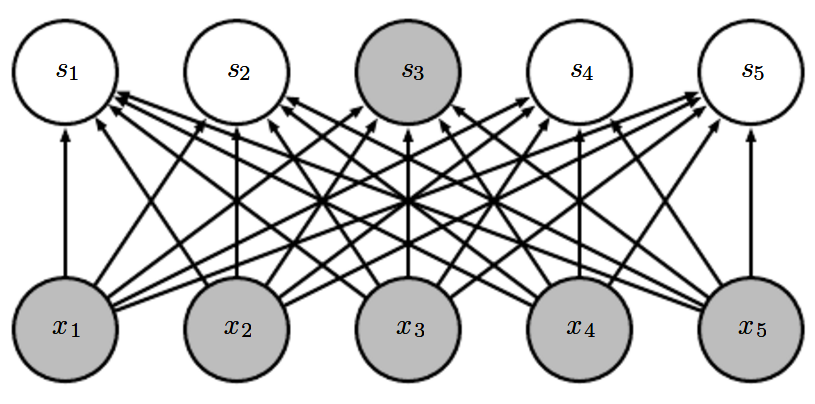
\includegraphics[width=.9\linewidth]{fig/full}
  \caption{Conectividade tradicional.}
  \label{fig:full}
\end{subfigure}%
\end{figure}

O \textbf{compartilhamento de parâmetros}, também chamado de \textbf{pesos amarrados},
se refere ao uso do mesmo parâmetro para mais de uma função no modelo.
Como já mencionado, nas redes neurais tradicionais todos os neurônios de uma camada são conectados a todos os neurônios
da camada anterior e cada neurônio possui um \textit{bias}, como ilustrado na imagem \ref{fig:shallow}.
Entretanto, este modelo é pouco eficiente, pois não tira vantagem da estruturas espaciais das imagens
de entrada \cite{Gdfl16}.
\begin{figure}[htp]
\begin{center}
  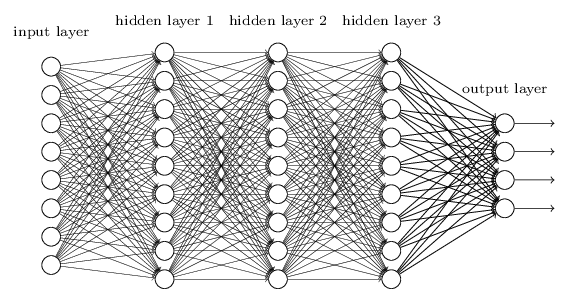
\includegraphics[width=0.7\textwidth]{fig/shallow_nn}
  \caption{Organização de camadas de uma rede neural do tipo \textit{feedforward}.}
  \label{fig:shallow}
\end{center}
\end{figure}
Estas informações estruturais são muito relevantes quando o problema em estudo é geoestatístico.
Por outro lado, no compartilhamento de pesos a saída de cada neurônio de uma camada depende apenas do conjunto de neurônios
de uma pequena região definida pelo campo receptivo da camada anterior:

\begin{equation}
 {\sigma} \times \bigg( b + \sum_{m}\sum_{n}{w_{m,n}a_{i+m,j+n} \bigg) }
\end{equation}
onde, $\sigma$ é uma função de ativação, $b$ é o valor compartilhado do \textit{bias}, $w_{m,n}$ é
uma matriz de pesos compartilhados (filtros) e $a_{i+m,j+n}$ denota a entrada $a_{x,y}$ na posição
$x,y$. Como o mesmo filtro é convolvido ao logo da imagem,
os mesmos pesos e \textit{bias} aprendem diferentes características da imagem. Deste modo, cada conjunto de pesos e \textit{bias} é compartilhado
por diferentes regiões em cada imagem e o número de pesos conectados ao neurônio
da camada seguinte diminui em relação ao modelo tradicional. Isto faz com que a convolução seja mais eficiente que a multiplicação de matriz
do ponto de vista de requisitos de memória e eficiência estatística.

O compartilhamento de pesos confere às redes convolucionais a propriedade de \textbf{equivariância} de
translação. Se uma função é equivariante, significa que se a entrada muda,
a saída muda igualmente. Matematicamente, a função $f(x)$ é equivariante à função $g$ se
$f(g(x)) = g(f(x))$. No caso da convolução, se $g$ é uma função que translada a entrada, então
a convolução será equivariante a $g$.
A convolução com imagens cria um mapa 2-D dos locais onde certas características aparecem na entrada.
A propriedade de equivariância permite rastrear objetos transladados na entrada. Se um objeto aparece
em uma determinada posição e, em seguida, aparece em outra posição, sua representação
irá mover a mesma quantidade na saída. É importante frisar que, nas CNN, a propriedade de equivariância
é aplicável apenas para a translação, de modo que a convolução não é equivariante para transformações 
de escala e rotações na imagem.

\section{Resumo}

Este Capítulo detalhou os principais conceitos abordados neste trabalho. O
problema inverso foi introduzido e a inversão sísmica apresentada em
maiores detalhes. Foram apresentados os elementos que compõem as redes
neurais convolucionais: a convolução, as camadas convolucionais, os filtros e a camada de \textit{pooling}.
Foram apresentadas também as propriedades das camadas convolucionais: conectividade esparsa,
compartilhamento de parâmetros, equivariância de translação, 